\documentclass[twoside]{book}

% Packages required by doxygen
\usepackage{fixltx2e}
\usepackage{calc}
\usepackage{doxygen}
\usepackage[export]{adjustbox} % also loads graphicx
\usepackage{graphicx}
\usepackage[utf8]{inputenc}
\usepackage{makeidx}
\usepackage{multicol}
\usepackage{multirow}
\PassOptionsToPackage{warn}{textcomp}
\usepackage{textcomp}
\usepackage[nointegrals]{wasysym}
\usepackage[table]{xcolor}

% Font selection
\usepackage[T1]{fontenc}
\usepackage[scaled=.90]{helvet}
\usepackage{courier}
\usepackage{amssymb}
\usepackage{sectsty}
\renewcommand{\familydefault}{\sfdefault}
\allsectionsfont{%
  \fontseries{bc}\selectfont%
  \color{darkgray}%
}
\renewcommand{\DoxyLabelFont}{%
  \fontseries{bc}\selectfont%
  \color{darkgray}%
}
\newcommand{\+}{\discretionary{\mbox{\scriptsize$\hookleftarrow$}}{}{}}

% Page & text layout
\usepackage{geometry}
\geometry{%
  a4paper,%
  top=2.5cm,%
  bottom=2.5cm,%
  left=2.5cm,%
  right=2.5cm%
}
\tolerance=750
\hfuzz=15pt
\hbadness=750
\setlength{\emergencystretch}{15pt}
\setlength{\parindent}{0cm}
\setlength{\parskip}{3ex plus 2ex minus 2ex}
\makeatletter
\renewcommand{\paragraph}{%
  \@startsection{paragraph}{4}{0ex}{-1.0ex}{1.0ex}{%
    \normalfont\normalsize\bfseries\SS@parafont%
  }%
}
\renewcommand{\subparagraph}{%
  \@startsection{subparagraph}{5}{0ex}{-1.0ex}{1.0ex}{%
    \normalfont\normalsize\bfseries\SS@subparafont%
  }%
}
\makeatother

% Headers & footers
\usepackage{fancyhdr}
\pagestyle{fancyplain}
\fancyhead[LE]{\fancyplain{}{\bfseries\thepage}}
\fancyhead[CE]{\fancyplain{}{}}
\fancyhead[RE]{\fancyplain{}{\bfseries\leftmark}}
\fancyhead[LO]{\fancyplain{}{\bfseries\rightmark}}
\fancyhead[CO]{\fancyplain{}{}}
\fancyhead[RO]{\fancyplain{}{\bfseries\thepage}}
\fancyfoot[LE]{\fancyplain{}{}}
\fancyfoot[CE]{\fancyplain{}{}}
\fancyfoot[RE]{\fancyplain{}{\bfseries\scriptsize Generated by Doxygen }}
\fancyfoot[LO]{\fancyplain{}{\bfseries\scriptsize Generated by Doxygen }}
\fancyfoot[CO]{\fancyplain{}{}}
\fancyfoot[RO]{\fancyplain{}{}}
\renewcommand{\footrulewidth}{0.4pt}
\renewcommand{\chaptermark}[1]{%
  \markboth{#1}{}%
}
\renewcommand{\sectionmark}[1]{%
  \markright{\thesection\ #1}%
}

% Indices & bibliography
\usepackage{natbib}
\usepackage[titles]{tocloft}
\setcounter{tocdepth}{3}
\setcounter{secnumdepth}{5}
\makeindex

% Custom commands
\newcommand{\clearemptydoublepage}{%
  \newpage{\pagestyle{empty}\cleardoublepage}%
}

\usepackage{caption}
\captionsetup{labelsep=space,justification=centering,font={bf},singlelinecheck=off,skip=4pt,position=top}

%===== C O N T E N T S =====

\begin{document}

% Titlepage & ToC
\pagenumbering{alph}
\begin{titlepage}
\vspace*{7cm}
\begin{center}%
{\Large P\+A5\+\_\+\+Mushatt }\\
\vspace*{1cm}
{\large Generated by Doxygen 1.8.13}\\
\end{center}
\end{titlepage}
\clearemptydoublepage
\pagenumbering{roman}
\tableofcontents
\clearemptydoublepage
\pagenumbering{arabic}

%--- Begin generated contents ---
\chapter{Hierarchical Index}
\section{Class Hierarchy}
This inheritance list is sorted roughly, but not completely, alphabetically\+:\begin{DoxyCompactList}
\item \contentsline{section}{Compare\+Event\+Time}{\pageref{classCompareEventTime}}{}
\item \contentsline{section}{Customer}{\pageref{classCustomer}}{}
\item \contentsline{section}{Event}{\pageref{classEvent}}{}
\begin{DoxyCompactList}
\item \contentsline{section}{Customer\+Event}{\pageref{classCustomerEvent}}{}
\item \contentsline{section}{Teller\+Event}{\pageref{classTellerEvent}}{}
\end{DoxyCompactList}
\item \contentsline{section}{Event\+Queue}{\pageref{classEventQueue}}{}
\item \contentsline{section}{Teller}{\pageref{classTeller}}{}
\item \contentsline{section}{Teller\+Queue}{\pageref{classTellerQueue}}{}
\end{DoxyCompactList}

\chapter{Class Index}
\section{Class List}
Here are the classes, structs, unions and interfaces with brief descriptions\+:\begin{DoxyCompactList}
\item\contentsline{section}{\textbf{ Customer} }{\pageref{classCustomer}}{}
\item\contentsline{section}{\textbf{ Customer\+Event} }{\pageref{classCustomerEvent}}{}
\item\contentsline{section}{\textbf{ Event} }{\pageref{classEvent}}{}
\item\contentsline{section}{\textbf{ Event\+Queue} }{\pageref{classEventQueue}}{}
\item\contentsline{section}{\textbf{ Teller} }{\pageref{classTeller}}{}
\item\contentsline{section}{\textbf{ Teller\+Event} }{\pageref{classTellerEvent}}{}
\item\contentsline{section}{\textbf{ Teller\+Queue} }{\pageref{classTellerQueue}}{}
\end{DoxyCompactList}

\chapter{File Index}
\section{File List}
Here is a list of all files with brief descriptions\+:\begin{DoxyCompactList}
\item\contentsline{section}{\textbf{ mystruct.\+c} }{\pageref{mystruct_8c}}{}
\item\contentsline{section}{\textbf{ mystruct.\+h} }{\pageref{mystruct_8h}}{}
\item\contentsline{section}{\textbf{ structest.\+c} }{\pageref{structest_8c}}{}
\end{DoxyCompactList}

\chapter{Class Documentation}
\section{Customer Class Reference}
\label{classCustomer}\index{Customer@{Customer}}


{\ttfamily \#include $<$Customer.\+h$>$}

\subsection*{Public Member Functions}
\begin{DoxyCompactItemize}
\item 
\textbf{ Customer} ()
\item 
virtual \textbf{ $\sim$\+Customer} ()
\item 
\textbf{ Customer} (\textbf{ Customer\+Event} $\ast$\textbf{ event})
\item 
void \textbf{ set\+Next\+Customer} (\textbf{ Customer} $\ast$cust)
\item 
\textbf{ Customer} $\ast$ \textbf{ get\+Next\+Customer} ()
\item 
\textbf{ Customer\+Event} $\ast$ \textbf{ get\+Customer\+Event} ()
\end{DoxyCompactItemize}
\subsection*{Public Attributes}
\begin{DoxyCompactItemize}
\item 
\textbf{ Customer} $\ast$ \textbf{ next\+Customer}
\item 
\textbf{ Customer\+Event} $\ast$ \textbf{ event}
\end{DoxyCompactItemize}


\subsection{Constructor \& Destructor Documentation}
\mbox{\label{classCustomer_abcc8fae9701e5ba9d7d6fe44498b34e3}} 
\index{Customer@{Customer}!Customer@{Customer}}
\index{Customer@{Customer}!Customer@{Customer}}
\subsubsection{Customer()\hspace{0.1cm}{\footnotesize\ttfamily [1/2]}}
{\footnotesize\ttfamily Customer\+::\+Customer (\begin{DoxyParamCaption}{ }\end{DoxyParamCaption})}

\mbox{\label{classCustomer_ab93fb14683b0393b9c900109f77c2629}} 
\index{Customer@{Customer}!````~Customer@{$\sim$\+Customer}}
\index{````~Customer@{$\sim$\+Customer}!Customer@{Customer}}
\subsubsection{$\sim$\+Customer()}
{\footnotesize\ttfamily Customer\+::$\sim$\+Customer (\begin{DoxyParamCaption}{ }\end{DoxyParamCaption})\hspace{0.3cm}{\ttfamily [virtual]}}

\mbox{\label{classCustomer_a4a0eb55dbdedb6be52d48a817a2d8f6f}} 
\index{Customer@{Customer}!Customer@{Customer}}
\index{Customer@{Customer}!Customer@{Customer}}
\subsubsection{Customer()\hspace{0.1cm}{\footnotesize\ttfamily [2/2]}}
{\footnotesize\ttfamily Customer\+::\+Customer (\begin{DoxyParamCaption}\item[{\textbf{ Customer\+Event} $\ast$}]{event }\end{DoxyParamCaption})}



References event, and next\+Customer.



\subsection{Member Function Documentation}
\mbox{\label{classCustomer_ae89a1bad867beae4d655a72eee491b32}} 
\index{Customer@{Customer}!get\+Customer\+Event@{get\+Customer\+Event}}
\index{get\+Customer\+Event@{get\+Customer\+Event}!Customer@{Customer}}
\subsubsection{get\+Customer\+Event()}
{\footnotesize\ttfamily \textbf{ Customer\+Event} $\ast$ Customer\+::get\+Customer\+Event (\begin{DoxyParamCaption}{ }\end{DoxyParamCaption})}

Retrieves the customer\textquotesingle{}s event \begin{DoxyReturn}{Returns}
Pointer to event 
\end{DoxyReturn}


References event.



Referenced by Teller\+Event\+::action(), and Teller\+Event\+::check\+Other\+Queues().

\mbox{\label{classCustomer_ae0e584d36211fad18ef0a99c828cec69}} 
\index{Customer@{Customer}!get\+Next\+Customer@{get\+Next\+Customer}}
\index{get\+Next\+Customer@{get\+Next\+Customer}!Customer@{Customer}}
\subsubsection{get\+Next\+Customer()}
{\footnotesize\ttfamily \textbf{ Customer} $\ast$ Customer\+::get\+Next\+Customer (\begin{DoxyParamCaption}{ }\end{DoxyParamCaption})}

Retrieve the next\+Customer \begin{DoxyReturn}{Returns}
Pointer to the next customer 
\end{DoxyReturn}


References next\+Customer.



Referenced by Teller\+Queue\+::remove\+Customer().

\mbox{\label{classCustomer_a677e901e3693e63519f03b08c0348f20}} 
\index{Customer@{Customer}!set\+Next\+Customer@{set\+Next\+Customer}}
\index{set\+Next\+Customer@{set\+Next\+Customer}!Customer@{Customer}}
\subsubsection{set\+Next\+Customer()}
{\footnotesize\ttfamily void Customer\+::set\+Next\+Customer (\begin{DoxyParamCaption}\item[{\textbf{ Customer} $\ast$}]{cust }\end{DoxyParamCaption})}

Set next\+Customer to cust 
\begin{DoxyParams}{Parameters}
{\em cust} & Pointer to new customer \\
\hline
\end{DoxyParams}


References next\+Customer.



Referenced by Teller\+Queue\+::add\+Customer().



\subsection{Member Data Documentation}
\mbox{\label{classCustomer_a671c01359a83ebbe7dfa31c796a1e766}} 
\index{Customer@{Customer}!event@{event}}
\index{event@{event}!Customer@{Customer}}
\subsubsection{event}
{\footnotesize\ttfamily \textbf{ Customer\+Event}$\ast$ Customer\+::event}



Referenced by Customer(), and get\+Customer\+Event().

\mbox{\label{classCustomer_a754b9aeb205889acaaef4cf253940fa6}} 
\index{Customer@{Customer}!next\+Customer@{next\+Customer}}
\index{next\+Customer@{next\+Customer}!Customer@{Customer}}
\subsubsection{next\+Customer}
{\footnotesize\ttfamily \textbf{ Customer}$\ast$ Customer\+::next\+Customer}



Referenced by Teller\+Queue\+::add\+Customer(), Customer(), get\+Next\+Customer(), and set\+Next\+Customer().



The documentation for this class was generated from the following files\+:\begin{DoxyCompactItemize}
\item 
\textbf{ Customer.\+h}\item 
\textbf{ Customer.\+cpp}\end{DoxyCompactItemize}

\section{Customer\+Event Class Reference}
\label{classCustomerEvent}\index{Customer\+Event@{Customer\+Event}}


{\ttfamily \#include $<$Customer\+Event.\+h$>$}

Inheritance diagram for Customer\+Event\+:\begin{figure}[H]
\begin{center}
\leavevmode
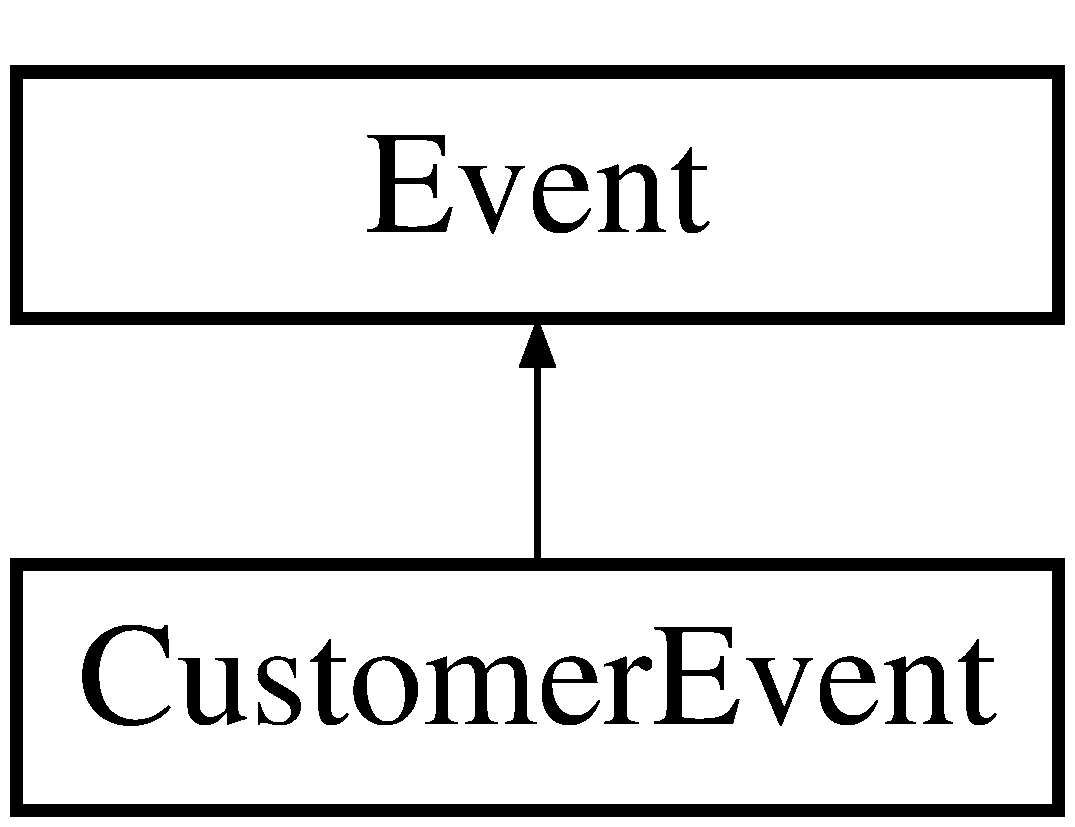
\includegraphics[height=2.000000cm]{classCustomerEvent}
\end{center}
\end{figure}
\subsection*{Public Member Functions}
\begin{DoxyCompactItemize}
\item 
\textbf{ Customer\+Event} (float \textbf{ start\+Time})
\item 
virtual \textbf{ $\sim$\+Customer\+Event} ()
\item 
void \textbf{ action} (float current\+Time, \textbf{ Teller\+Queue} $\ast$$\ast$queues, int num\+Tellers, \textbf{ Event\+Queue} $\ast$simulation\+Queue)
\item 
float \textbf{ get\+Time} ()
\item 
void \textbf{ set\+Service} ()
\item 
void \textbf{ set\+Time} (float t)
\item 
bool \textbf{ get\+Servicing} ()
\item 
int \textbf{ get\+End\+Time} ()
\item 
int \textbf{ get\+Start\+Time} ()
\item 
\textbf{ Teller\+Queue} $\ast$ \textbf{ find\+Shortest\+Line} (\textbf{ Teller\+Queue} $\ast$$\ast$q, int num\+Tellers)
\end{DoxyCompactItemize}
\subsection*{Private Attributes}
\begin{DoxyCompactItemize}
\item 
float \textbf{ start\+Time}
\item 
float \textbf{ time}
\item 
float \textbf{ end\+Time}
\item 
bool \textbf{ receiving\+Service}
\end{DoxyCompactItemize}


\subsection{Constructor \& Destructor Documentation}
\mbox{\label{classCustomerEvent_aa300aafafb36b5bf46de53cb6ac534ff}} 
\index{Customer\+Event@{Customer\+Event}!Customer\+Event@{Customer\+Event}}
\index{Customer\+Event@{Customer\+Event}!Customer\+Event@{Customer\+Event}}
\subsubsection{Customer\+Event()}
{\footnotesize\ttfamily Customer\+Event\+::\+Customer\+Event (\begin{DoxyParamCaption}\item[{float}]{beginning\+Time }\end{DoxyParamCaption})}

Constructor 
\begin{DoxyParams}{Parameters}
{\em beginning\+Time} & Start time for the event \\
\hline
\end{DoxyParams}


References end\+Time, receiving\+Service, start\+Time, and time.

\mbox{\label{classCustomerEvent_ab437d164de7f6b27545e6b8c282037a6}} 
\index{Customer\+Event@{Customer\+Event}!````~Customer\+Event@{$\sim$\+Customer\+Event}}
\index{````~Customer\+Event@{$\sim$\+Customer\+Event}!Customer\+Event@{Customer\+Event}}
\subsubsection{$\sim$\+Customer\+Event()}
{\footnotesize\ttfamily Customer\+Event\+::$\sim$\+Customer\+Event (\begin{DoxyParamCaption}{ }\end{DoxyParamCaption})\hspace{0.3cm}{\ttfamily [virtual]}}



\subsection{Member Function Documentation}
\mbox{\label{classCustomerEvent_a4b065700b1edb402328a4328ed4b7ea2}} 
\index{Customer\+Event@{Customer\+Event}!action@{action}}
\index{action@{action}!Customer\+Event@{Customer\+Event}}
\subsubsection{action()}
{\footnotesize\ttfamily void Customer\+Event\+::action (\begin{DoxyParamCaption}\item[{float}]{current\+Time,  }\item[{\textbf{ Teller\+Queue} $\ast$$\ast$}]{queues,  }\item[{int}]{num\+Tellers,  }\item[{\textbf{ Event\+Queue} $\ast$}]{simulation\+Queue }\end{DoxyParamCaption})\hspace{0.3cm}{\ttfamily [virtual]}}

The action to be called on by the \doxyref{Event}{p.}{classEvent} Queue 
\begin{DoxyParams}{Parameters}
{\em current\+Time} & time to update end\+Time \\
\hline
{\em queues} & \doxyref{Teller}{p.}{classTeller} queues to check/use \\
\hline
{\em num\+Tellers} & \# of teller queues \\
\hline
{\em simulation\+Queue} & \doxyref{Event}{p.}{classEvent} Queue to update for action \\
\hline
\end{DoxyParams}


Reimplemented from \textbf{ Event} \doxyref{}{p.}{classEvent_aa37a026dd3cb09ab57f80b8817d0c1bc}.



References Teller\+Queue\+::add\+Customer(), end\+Time, find\+Shortest\+Line(), receiving\+Service, and Event\+Queue\+::remove\+Event().

\mbox{\label{classCustomerEvent_a7acf9da15cfade2cfd1cf3d1d8719f2e}} 
\index{Customer\+Event@{Customer\+Event}!find\+Shortest\+Line@{find\+Shortest\+Line}}
\index{find\+Shortest\+Line@{find\+Shortest\+Line}!Customer\+Event@{Customer\+Event}}
\subsubsection{find\+Shortest\+Line()}
{\footnotesize\ttfamily \textbf{ Teller\+Queue} $\ast$ Customer\+Event\+::find\+Shortest\+Line (\begin{DoxyParamCaption}\item[{\textbf{ Teller\+Queue} $\ast$$\ast$}]{lines,  }\item[{int}]{num\+Lines }\end{DoxyParamCaption})}

Retrieve the shortest line amongt a 2d array of tellerqueues 
\begin{DoxyParams}{Parameters}
{\em lines} & Pointer to teller queues \\
\hline
{\em num\+Lines} & \# of teller queues \\
\hline
\end{DoxyParams}
\begin{DoxyReturn}{Returns}
The shortest line 
\end{DoxyReturn}


References Teller\+Queue\+::get\+Queue\+Size().



Referenced by action().

\mbox{\label{classCustomerEvent_a86f2e7ca538c0a989b5c314c0e5e8be0}} 
\index{Customer\+Event@{Customer\+Event}!get\+End\+Time@{get\+End\+Time}}
\index{get\+End\+Time@{get\+End\+Time}!Customer\+Event@{Customer\+Event}}
\subsubsection{get\+End\+Time()}
{\footnotesize\ttfamily int Customer\+Event\+::get\+End\+Time (\begin{DoxyParamCaption}{ }\end{DoxyParamCaption})}

Retrieve end time \begin{DoxyReturn}{Returns}
end time for the event 
\end{DoxyReturn}


References end\+Time.



Referenced by run\+Sim().

\mbox{\label{classCustomerEvent_aeeaa7c12449ac5074797d97cb0af84d8}} 
\index{Customer\+Event@{Customer\+Event}!get\+Servicing@{get\+Servicing}}
\index{get\+Servicing@{get\+Servicing}!Customer\+Event@{Customer\+Event}}
\subsubsection{get\+Servicing()}
{\footnotesize\ttfamily bool Customer\+Event\+::get\+Servicing (\begin{DoxyParamCaption}{ }\end{DoxyParamCaption})}

Retrieve service status \begin{DoxyReturn}{Returns}
True if processed, false if unprocessed 
\end{DoxyReturn}


References receiving\+Service.

\mbox{\label{classCustomerEvent_aba4cde0a8f57d3b87f61cc1b011e8aa4}} 
\index{Customer\+Event@{Customer\+Event}!get\+Start\+Time@{get\+Start\+Time}}
\index{get\+Start\+Time@{get\+Start\+Time}!Customer\+Event@{Customer\+Event}}
\subsubsection{get\+Start\+Time()}
{\footnotesize\ttfamily int Customer\+Event\+::get\+Start\+Time (\begin{DoxyParamCaption}{ }\end{DoxyParamCaption})}

Retrieve start Time \begin{DoxyReturn}{Returns}
start time for event 
\end{DoxyReturn}


References start\+Time.



Referenced by run\+Sim().

\mbox{\label{classCustomerEvent_acfcd323cd02d825bc0095a07947cf10b}} 
\index{Customer\+Event@{Customer\+Event}!get\+Time@{get\+Time}}
\index{get\+Time@{get\+Time}!Customer\+Event@{Customer\+Event}}
\subsubsection{get\+Time()}
{\footnotesize\ttfamily float Customer\+Event\+::get\+Time (\begin{DoxyParamCaption}{ }\end{DoxyParamCaption})\hspace{0.3cm}{\ttfamily [virtual]}}

Retreieve event time \begin{DoxyReturn}{Returns}
event time 
\end{DoxyReturn}


Reimplemented from \textbf{ Event} \doxyref{}{p.}{classEvent_af56f6b60a3c1ce8d954e13ce4ad54dc2}.



References time.

\mbox{\label{classCustomerEvent_a28a3232371c5cdea52eb4b816c1304a4}} 
\index{Customer\+Event@{Customer\+Event}!set\+Service@{set\+Service}}
\index{set\+Service@{set\+Service}!Customer\+Event@{Customer\+Event}}
\subsubsection{set\+Service()}
{\footnotesize\ttfamily void Customer\+Event\+::set\+Service (\begin{DoxyParamCaption}{ }\end{DoxyParamCaption})}

Set whether this event has been processed by a teller 

References receiving\+Service.



Referenced by Teller\+Event\+::action().

\mbox{\label{classCustomerEvent_a6849292c3e45902a3e22d1ccbe45f61d}} 
\index{Customer\+Event@{Customer\+Event}!set\+Time@{set\+Time}}
\index{set\+Time@{set\+Time}!Customer\+Event@{Customer\+Event}}
\subsubsection{set\+Time()}
{\footnotesize\ttfamily void Customer\+Event\+::set\+Time (\begin{DoxyParamCaption}\item[{float}]{current\+Time }\end{DoxyParamCaption})}

Update the events current time 
\begin{DoxyParams}{Parameters}
{\em current\+Time} & Time to update to \\
\hline
\end{DoxyParams}


References time.



Referenced by Teller\+Event\+::action().



\subsection{Member Data Documentation}
\mbox{\label{classCustomerEvent_a9e6b36c6033458c706784ff2ce40ed52}} 
\index{Customer\+Event@{Customer\+Event}!end\+Time@{end\+Time}}
\index{end\+Time@{end\+Time}!Customer\+Event@{Customer\+Event}}
\subsubsection{end\+Time}
{\footnotesize\ttfamily float Customer\+Event\+::end\+Time\hspace{0.3cm}{\ttfamily [private]}}



Referenced by action(), Customer\+Event(), and get\+End\+Time().

\mbox{\label{classCustomerEvent_a3c3c75c8ef27ee0d93d58496a7230fc2}} 
\index{Customer\+Event@{Customer\+Event}!receiving\+Service@{receiving\+Service}}
\index{receiving\+Service@{receiving\+Service}!Customer\+Event@{Customer\+Event}}
\subsubsection{receiving\+Service}
{\footnotesize\ttfamily bool Customer\+Event\+::receiving\+Service\hspace{0.3cm}{\ttfamily [private]}}



Referenced by action(), Customer\+Event(), get\+Servicing(), and set\+Service().

\mbox{\label{classCustomerEvent_a5a461d610547755fe4b7fdc27b4d9db7}} 
\index{Customer\+Event@{Customer\+Event}!start\+Time@{start\+Time}}
\index{start\+Time@{start\+Time}!Customer\+Event@{Customer\+Event}}
\subsubsection{start\+Time}
{\footnotesize\ttfamily float Customer\+Event\+::start\+Time\hspace{0.3cm}{\ttfamily [private]}}



Referenced by Customer\+Event(), and get\+Start\+Time().

\mbox{\label{classCustomerEvent_a896c4f12de76d072078dac50788c790b}} 
\index{Customer\+Event@{Customer\+Event}!time@{time}}
\index{time@{time}!Customer\+Event@{Customer\+Event}}
\subsubsection{time}
{\footnotesize\ttfamily float Customer\+Event\+::time\hspace{0.3cm}{\ttfamily [private]}}



Referenced by Customer\+Event(), get\+Time(), and set\+Time().



The documentation for this class was generated from the following files\+:\begin{DoxyCompactItemize}
\item 
\textbf{ Customer\+Event.\+h}\item 
\textbf{ Customer\+Event.\+cpp}\end{DoxyCompactItemize}

\section{Event Class Reference}
\label{classEvent}\index{Event@{Event}}


{\ttfamily \#include $<$Event.\+h$>$}

Inheritance diagram for Event\+:\begin{figure}[H]
\begin{center}
\leavevmode
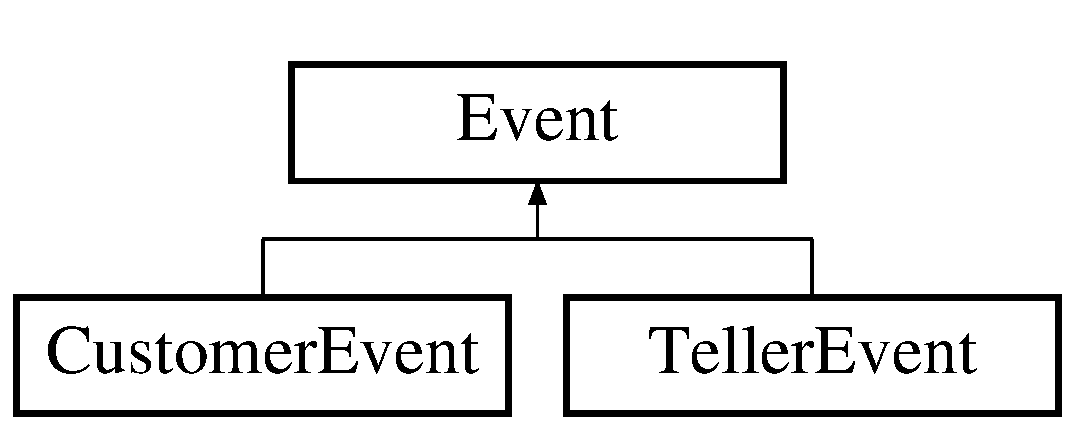
\includegraphics[height=2.000000cm]{classEvent}
\end{center}
\end{figure}
\subsection*{Public Member Functions}
\begin{DoxyCompactItemize}
\item 
\textbf{ Event} ()
\item 
virtual \textbf{ $\sim$\+Event} ()
\item 
virtual float \textbf{ get\+Time} ()
\item 
virtual void \textbf{ action} (float current\+Time, \textbf{ Teller\+Queue} $\ast$$\ast$queues, int num\+Tellers, \textbf{ Event\+Queue} $\ast$simulation\+Queue)
\item 
\textbf{ Event} $\ast$ \textbf{ get\+Next\+Event} ()
\item 
void \textbf{ set\+Next} (\textbf{ Event} $\ast$event)
\end{DoxyCompactItemize}
\subsection*{Private Attributes}
\begin{DoxyCompactItemize}
\item 
float \textbf{ time}
\item 
\textbf{ Event} $\ast$ \textbf{ next\+Event}
\end{DoxyCompactItemize}


\subsection{Constructor \& Destructor Documentation}
\mbox{\label{classEvent_a5a40dd4708297f7031e29b39e039ae10}} 
\index{Event@{Event}!Event@{Event}}
\index{Event@{Event}!Event@{Event}}
\subsubsection{Event()}
{\footnotesize\ttfamily Event\+::\+Event (\begin{DoxyParamCaption}{ }\end{DoxyParamCaption})}

Constructor for event 

References next\+Event, and time.

\mbox{\label{classEvent_a7704ec01ce91e673885792054214b3d2}} 
\index{Event@{Event}!````~Event@{$\sim$\+Event}}
\index{````~Event@{$\sim$\+Event}!Event@{Event}}
\subsubsection{$\sim$\+Event()}
{\footnotesize\ttfamily Event\+::$\sim$\+Event (\begin{DoxyParamCaption}{ }\end{DoxyParamCaption})\hspace{0.3cm}{\ttfamily [virtual]}}



\subsection{Member Function Documentation}
\mbox{\label{classEvent_aa37a026dd3cb09ab57f80b8817d0c1bc}} 
\index{Event@{Event}!action@{action}}
\index{action@{action}!Event@{Event}}
\subsubsection{action()}
{\footnotesize\ttfamily void Event\+::action (\begin{DoxyParamCaption}\item[{float}]{current\+Time,  }\item[{\textbf{ Teller\+Queue} $\ast$$\ast$}]{queues,  }\item[{int}]{num\+Tellers,  }\item[{\textbf{ Event\+Queue} $\ast$}]{simulation\+Queue }\end{DoxyParamCaption})\hspace{0.3cm}{\ttfamily [virtual]}}

Action for the event, to be overriden by subclasses 
\begin{DoxyParams}{Parameters}
{\em current\+Time} & Current sim time \\
\hline
{\em queues} & \doxyref{Teller}{p.}{classTeller} queues \\
\hline
{\em num\+Tellers} & \# of tellers \\
\hline
{\em simulation\+Queue} & \doxyref{Event}{p.}{classEvent} Queue \\
\hline
\end{DoxyParams}


Reimplemented in \textbf{ Teller\+Event} \doxyref{}{p.}{classTellerEvent_a718d62796e9e8cda1f6b44e2001416ba}, and \textbf{ Customer\+Event} \doxyref{}{p.}{classCustomerEvent_a4b065700b1edb402328a4328ed4b7ea2}.

\mbox{\label{classEvent_a72121dab5e403605b1f0e0f82ca375f9}} 
\index{Event@{Event}!get\+Next\+Event@{get\+Next\+Event}}
\index{get\+Next\+Event@{get\+Next\+Event}!Event@{Event}}
\subsubsection{get\+Next\+Event()}
{\footnotesize\ttfamily \textbf{ Event} $\ast$ Event\+::get\+Next\+Event (\begin{DoxyParamCaption}{ }\end{DoxyParamCaption})}

Retrieve the next event \begin{DoxyReturn}{Returns}
The next event 
\end{DoxyReturn}


References next\+Event.



Referenced by Event\+Queue\+::add\+Event(), Event\+Queue\+::get\+Event\+At(), and Event\+Queue\+::remove\+Event().

\mbox{\label{classEvent_af56f6b60a3c1ce8d954e13ce4ad54dc2}} 
\index{Event@{Event}!get\+Time@{get\+Time}}
\index{get\+Time@{get\+Time}!Event@{Event}}
\subsubsection{get\+Time()}
{\footnotesize\ttfamily float Event\+::get\+Time (\begin{DoxyParamCaption}{ }\end{DoxyParamCaption})\hspace{0.3cm}{\ttfamily [virtual]}}

Retrieve time for the event \begin{DoxyReturn}{Returns}
time of the event 
\end{DoxyReturn}


Reimplemented in \textbf{ Teller\+Event} \doxyref{}{p.}{classTellerEvent_a9d00862b1033b7f11616071e8294d97b}, and \textbf{ Customer\+Event} \doxyref{}{p.}{classCustomerEvent_acfcd323cd02d825bc0095a07947cf10b}.



References time.



Referenced by Event\+Queue\+::add\+Event(), and run\+Sim().

\mbox{\label{classEvent_afe191087bacd061d2f8e4620b4442609}} 
\index{Event@{Event}!set\+Next@{set\+Next}}
\index{set\+Next@{set\+Next}!Event@{Event}}
\subsubsection{set\+Next()}
{\footnotesize\ttfamily void Event\+::set\+Next (\begin{DoxyParamCaption}\item[{\textbf{ Event} $\ast$}]{event }\end{DoxyParamCaption})}

Set the next event for the current event 
\begin{DoxyParams}{Parameters}
{\em event} & Pointer to event to update to \\
\hline
\end{DoxyParams}


References next\+Event.



Referenced by Event\+Queue\+::add\+Event().



\subsection{Member Data Documentation}
\mbox{\label{classEvent_ad4703fce68801b81600587e72385e3ab}} 
\index{Event@{Event}!next\+Event@{next\+Event}}
\index{next\+Event@{next\+Event}!Event@{Event}}
\subsubsection{next\+Event}
{\footnotesize\ttfamily \textbf{ Event}$\ast$ Event\+::next\+Event\hspace{0.3cm}{\ttfamily [private]}}



Referenced by Event(), get\+Next\+Event(), and set\+Next().

\mbox{\label{classEvent_a5b2142bf788396f92f36cb596b7c1e3c}} 
\index{Event@{Event}!time@{time}}
\index{time@{time}!Event@{Event}}
\subsubsection{time}
{\footnotesize\ttfamily float Event\+::time\hspace{0.3cm}{\ttfamily [private]}}



Referenced by Event(), and get\+Time().



The documentation for this class was generated from the following files\+:\begin{DoxyCompactItemize}
\item 
\textbf{ Event.\+h}\item 
\textbf{ Event.\+cpp}\end{DoxyCompactItemize}

\section{Event\+Queue Class Reference}
\label{classEventQueue}\index{Event\+Queue@{Event\+Queue}}


{\ttfamily \#include $<$Event\+Queue.\+h$>$}

\subsection*{Public Member Functions}
\begin{DoxyCompactItemize}
\item 
\textbf{ Event\+Queue} ()
\item 
virtual \textbf{ $\sim$\+Event\+Queue} ()
\item 
\textbf{ Event} $\ast$ \textbf{ get\+Head} ()
\item 
void \textbf{ remove\+Event} ()
\item 
void \textbf{ add\+Event} (\textbf{ Event} $\ast$event)
\item 
int \textbf{ get\+Queue\+Size} ()
\item 
\textbf{ Event} $\ast$ \textbf{ get\+Event\+At} (int index)
\end{DoxyCompactItemize}
\subsection*{Public Attributes}
\begin{DoxyCompactItemize}
\item 
std\+::priority\+\_\+queue$<$ \textbf{ Event} $\ast$, std\+::vector$<$ \textbf{ Event} $\ast$ $>$, \textbf{ Compare\+Event\+Time} $>$ \textbf{ p\+Queue}
\end{DoxyCompactItemize}


\subsection{Constructor \& Destructor Documentation}
\mbox{\label{classEventQueue_ab7de5a41befc94aac0f461391e67f14a}} 
\index{Event\+Queue@{Event\+Queue}!Event\+Queue@{Event\+Queue}}
\index{Event\+Queue@{Event\+Queue}!Event\+Queue@{Event\+Queue}}
\subsubsection{Event\+Queue()}
{\footnotesize\ttfamily Event\+Queue\+::\+Event\+Queue (\begin{DoxyParamCaption}{ }\end{DoxyParamCaption})}

Constructor, set head to nullptr and size to 0 \mbox{\label{classEventQueue_ac57db8e2366f2c6c594e6afc975e3b59}} 
\index{Event\+Queue@{Event\+Queue}!````~Event\+Queue@{$\sim$\+Event\+Queue}}
\index{````~Event\+Queue@{$\sim$\+Event\+Queue}!Event\+Queue@{Event\+Queue}}
\subsubsection{$\sim$\+Event\+Queue()}
{\footnotesize\ttfamily Event\+Queue\+::$\sim$\+Event\+Queue (\begin{DoxyParamCaption}{ }\end{DoxyParamCaption})\hspace{0.3cm}{\ttfamily [virtual]}}



\subsection{Member Function Documentation}
\mbox{\label{classEventQueue_a55e0d159086c702174a66e18dea05b78}} 
\index{Event\+Queue@{Event\+Queue}!add\+Event@{add\+Event}}
\index{add\+Event@{add\+Event}!Event\+Queue@{Event\+Queue}}
\subsubsection{add\+Event()}
{\footnotesize\ttfamily void Event\+Queue\+::add\+Event (\begin{DoxyParamCaption}\item[{\textbf{ Event} $\ast$}]{event }\end{DoxyParamCaption})}

Add event to the queue 
\begin{DoxyParams}{Parameters}
{\em event} & Pointer to event to add \\
\hline
\end{DoxyParams}


References p\+Queue.



Referenced by Teller\+Event\+::action(), and main().

\mbox{\label{classEventQueue_ab825fbc68ac03236a8c88c024ee6f81d}} 
\index{Event\+Queue@{Event\+Queue}!get\+Event\+At@{get\+Event\+At}}
\index{get\+Event\+At@{get\+Event\+At}!Event\+Queue@{Event\+Queue}}
\subsubsection{get\+Event\+At()}
{\footnotesize\ttfamily \textbf{ Event}$\ast$ Event\+Queue\+::get\+Event\+At (\begin{DoxyParamCaption}\item[{int}]{index }\end{DoxyParamCaption})}

\mbox{\label{classEventQueue_a22247fa958f0f7c59c6efa4221cec086}} 
\index{Event\+Queue@{Event\+Queue}!get\+Head@{get\+Head}}
\index{get\+Head@{get\+Head}!Event\+Queue@{Event\+Queue}}
\subsubsection{get\+Head()}
{\footnotesize\ttfamily \textbf{ Event} $\ast$ Event\+Queue\+::get\+Head (\begin{DoxyParamCaption}{ }\end{DoxyParamCaption})}

Retrieve the head of the event queue \begin{DoxyReturn}{Returns}
head/1st of event queue 
\end{DoxyReturn}


References p\+Queue.



Referenced by run\+Sim().

\mbox{\label{classEventQueue_a1657a805dc38663bbdca6996f1f75ec0}} 
\index{Event\+Queue@{Event\+Queue}!get\+Queue\+Size@{get\+Queue\+Size}}
\index{get\+Queue\+Size@{get\+Queue\+Size}!Event\+Queue@{Event\+Queue}}
\subsubsection{get\+Queue\+Size()}
{\footnotesize\ttfamily int Event\+Queue\+::get\+Queue\+Size (\begin{DoxyParamCaption}{ }\end{DoxyParamCaption})}

Retrieve queue size \begin{DoxyReturn}{Returns}
size of event queue 
\end{DoxyReturn}


References p\+Queue.



Referenced by run\+Sim().

\mbox{\label{classEventQueue_ac8b2d6de9e9275356fe893950f26a84b}} 
\index{Event\+Queue@{Event\+Queue}!remove\+Event@{remove\+Event}}
\index{remove\+Event@{remove\+Event}!Event\+Queue@{Event\+Queue}}
\subsubsection{remove\+Event()}
{\footnotesize\ttfamily void Event\+Queue\+::remove\+Event (\begin{DoxyParamCaption}{ }\end{DoxyParamCaption})}

Remove event from the event queue 

References p\+Queue.



Referenced by Customer\+Event\+::action(), and Teller\+Event\+::action().



\subsection{Member Data Documentation}
\mbox{\label{classEventQueue_a89681bfba67cfbdb7678e19b9a88a3e6}} 
\index{Event\+Queue@{Event\+Queue}!p\+Queue@{p\+Queue}}
\index{p\+Queue@{p\+Queue}!Event\+Queue@{Event\+Queue}}
\subsubsection{p\+Queue}
{\footnotesize\ttfamily std\+::priority\+\_\+queue$<$\textbf{ Event} $\ast$,std\+::vector$<$\textbf{ Event} $\ast$$>$,\textbf{ Compare\+Event\+Time}$>$ Event\+Queue\+::p\+Queue}



Referenced by add\+Event(), get\+Head(), get\+Queue\+Size(), and remove\+Event().



The documentation for this class was generated from the following files\+:\begin{DoxyCompactItemize}
\item 
\textbf{ Event\+Queue.\+h}\item 
\textbf{ Event\+Queue.\+cpp}\end{DoxyCompactItemize}

\section{Teller Class Reference}
\label{classTeller}\index{Teller@{Teller}}


{\ttfamily \#include $<$Teller.\+h$>$}

\subsection*{Public Member Functions}
\begin{DoxyCompactItemize}
\item 
\textbf{ Teller} (int num)
\item 
virtual \textbf{ $\sim$\+Teller} ()
\item 
void \textbf{ update\+Break\+Status} (\textbf{ Teller\+Queue} $\ast$line)
\item 
int \textbf{ get\+Idle\+Time} ()
\end{DoxyCompactItemize}
\subsection*{Public Attributes}
\begin{DoxyCompactItemize}
\item 
bool \textbf{ on\+Break}
\item 
bool \textbf{ processing}
\item 
int \textbf{ teller\+Num}
\end{DoxyCompactItemize}
\subsection*{Private Member Functions}
\begin{DoxyCompactItemize}
\item 
void \textbf{ set\+Idle\+Time} ()
\end{DoxyCompactItemize}
\subsection*{Private Attributes}
\begin{DoxyCompactItemize}
\item 
const int \textbf{ idle\+Time\+Const} = 600
\item 
int \textbf{ idle\+Time}
\end{DoxyCompactItemize}


\subsection{Constructor \& Destructor Documentation}
\mbox{\label{classTeller_a2ccfea7e98471237ffdc68687cf38970}} 
\index{Teller@{Teller}!Teller@{Teller}}
\index{Teller@{Teller}!Teller@{Teller}}
\subsubsection{Teller()}
{\footnotesize\ttfamily Teller\+::\+Teller (\begin{DoxyParamCaption}\item[{int}]{num }\end{DoxyParamCaption})}



References on\+Break, processing, set\+Idle\+Time(), and teller\+Num.

\mbox{\label{classTeller_af61263c98d7ff236ca84ec551919d7e7}} 
\index{Teller@{Teller}!````~Teller@{$\sim$\+Teller}}
\index{````~Teller@{$\sim$\+Teller}!Teller@{Teller}}
\subsubsection{$\sim$\+Teller()}
{\footnotesize\ttfamily Teller\+::$\sim$\+Teller (\begin{DoxyParamCaption}{ }\end{DoxyParamCaption})\hspace{0.3cm}{\ttfamily [virtual]}}



\subsection{Member Function Documentation}
\mbox{\label{classTeller_a4882535d0d135ba1ae02d83dce94b154}} 
\index{Teller@{Teller}!get\+Idle\+Time@{get\+Idle\+Time}}
\index{get\+Idle\+Time@{get\+Idle\+Time}!Teller@{Teller}}
\subsubsection{get\+Idle\+Time()}
{\footnotesize\ttfamily int Teller\+::get\+Idle\+Time (\begin{DoxyParamCaption}{ }\end{DoxyParamCaption})}

Returns idle time of teller \begin{DoxyReturn}{Returns}
Time to idlek 
\end{DoxyReturn}


References idle\+Time.

\mbox{\label{classTeller_a680268b558b302851143234261b33ac7}} 
\index{Teller@{Teller}!set\+Idle\+Time@{set\+Idle\+Time}}
\index{set\+Idle\+Time@{set\+Idle\+Time}!Teller@{Teller}}
\subsubsection{set\+Idle\+Time()}
{\footnotesize\ttfamily void Teller\+::set\+Idle\+Time (\begin{DoxyParamCaption}{ }\end{DoxyParamCaption})\hspace{0.3cm}{\ttfamily [private]}}

Sets idle time of teller 

References idle\+Time.



Referenced by Teller().

\mbox{\label{classTeller_ac2631da9a56456deb4a91a1a78b3cd1e}} 
\index{Teller@{Teller}!update\+Break\+Status@{update\+Break\+Status}}
\index{update\+Break\+Status@{update\+Break\+Status}!Teller@{Teller}}
\subsubsection{update\+Break\+Status()}
{\footnotesize\ttfamily void Teller\+::update\+Break\+Status (\begin{DoxyParamCaption}\item[{\textbf{ Teller\+Queue} $\ast$}]{line }\end{DoxyParamCaption})}

Check if the teller has any customers in some queue before changing idle status 
\begin{DoxyParams}{Parameters}
{\em $\ast$line} & Pointer to tellerqueue \\
\hline
\end{DoxyParams}


References Teller\+Queue\+::get\+Head(), and on\+Break.



\subsection{Member Data Documentation}
\mbox{\label{classTeller_a09db98c5db957cd1937b3b5e9fa2820b}} 
\index{Teller@{Teller}!idle\+Time@{idle\+Time}}
\index{idle\+Time@{idle\+Time}!Teller@{Teller}}
\subsubsection{idle\+Time}
{\footnotesize\ttfamily int Teller\+::idle\+Time\hspace{0.3cm}{\ttfamily [private]}}



Referenced by get\+Idle\+Time(), and set\+Idle\+Time().

\mbox{\label{classTeller_ac2dc8cb04d87147182cc565b0dbb2804}} 
\index{Teller@{Teller}!idle\+Time\+Const@{idle\+Time\+Const}}
\index{idle\+Time\+Const@{idle\+Time\+Const}!Teller@{Teller}}
\subsubsection{idle\+Time\+Const}
{\footnotesize\ttfamily const int Teller\+::idle\+Time\+Const = 600\hspace{0.3cm}{\ttfamily [private]}}

\mbox{\label{classTeller_a5d1b1edd74ced9664cbf19dd40256a5a}} 
\index{Teller@{Teller}!on\+Break@{on\+Break}}
\index{on\+Break@{on\+Break}!Teller@{Teller}}
\subsubsection{on\+Break}
{\footnotesize\ttfamily bool Teller\+::on\+Break}



Referenced by Teller(), and update\+Break\+Status().

\mbox{\label{classTeller_aa32cd13ff1cbd061a9765fac2f4b5450}} 
\index{Teller@{Teller}!processing@{processing}}
\index{processing@{processing}!Teller@{Teller}}
\subsubsection{processing}
{\footnotesize\ttfamily bool Teller\+::processing}



Referenced by Teller().

\mbox{\label{classTeller_a41aed4c5f9440b1dcfa07420a6908f68}} 
\index{Teller@{Teller}!teller\+Num@{teller\+Num}}
\index{teller\+Num@{teller\+Num}!Teller@{Teller}}
\subsubsection{teller\+Num}
{\footnotesize\ttfamily int Teller\+::teller\+Num}



Referenced by Teller().



The documentation for this class was generated from the following files\+:\begin{DoxyCompactItemize}
\item 
\textbf{ Teller.\+h}\item 
\textbf{ Teller.\+cpp}\end{DoxyCompactItemize}

\section{Teller\+Event Class Reference}
\label{classTellerEvent}\index{Teller\+Event@{Teller\+Event}}


{\ttfamily \#include $<$Teller\+Event.\+h$>$}

Inheritance diagram for Teller\+Event\+:\begin{figure}[H]
\begin{center}
\leavevmode
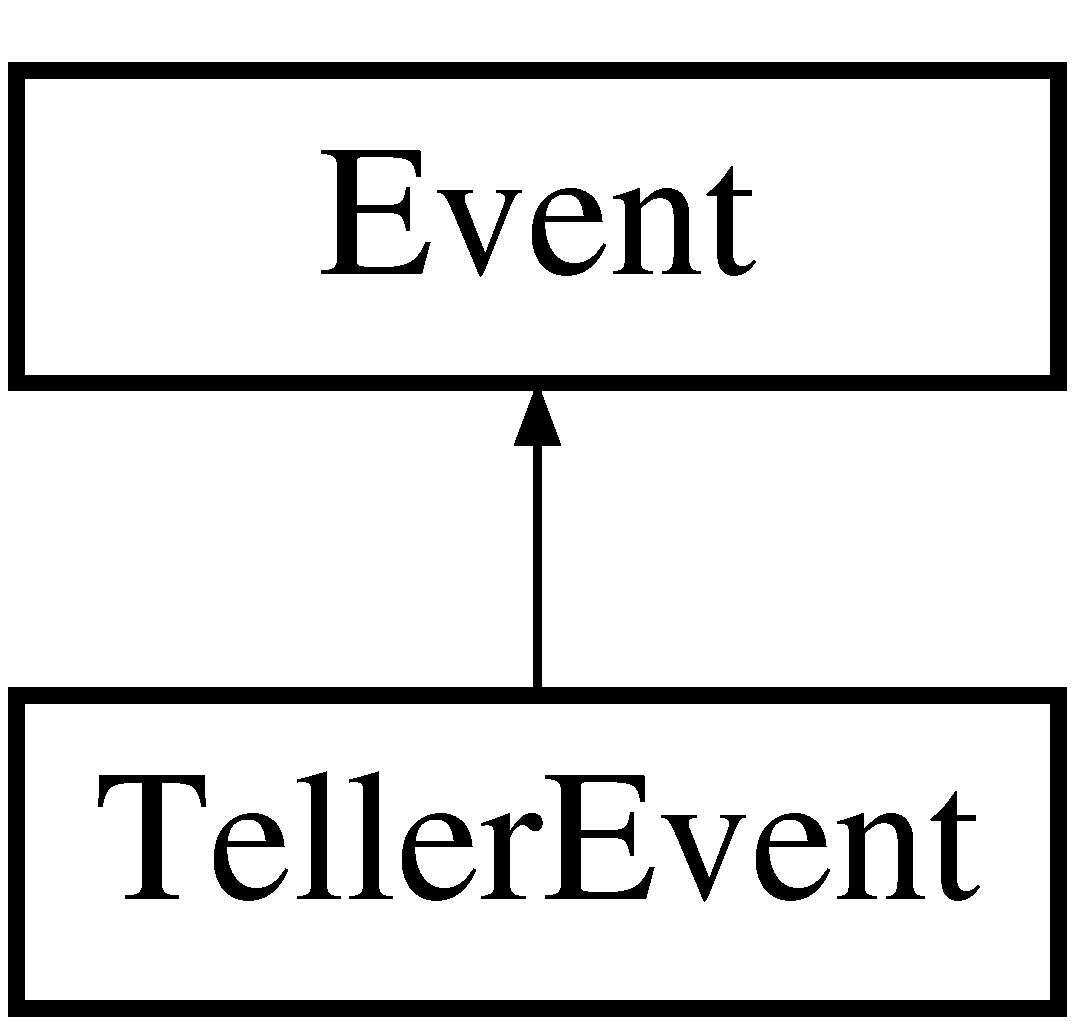
\includegraphics[height=2.000000cm]{classTellerEvent}
\end{center}
\end{figure}
\subsection*{Public Member Functions}
\begin{DoxyCompactItemize}
\item 
\textbf{ Teller\+Event} (float \textbf{ teller\+Service\+Time}, float \textbf{ idle\+Time}, \textbf{ Teller\+Queue} $\ast$\textbf{ queue})
\item 
virtual \textbf{ $\sim$\+Teller\+Event} ()
\item 
void \textbf{ action} (float current\+Time, \textbf{ Teller\+Queue} $\ast$$\ast$queues, int num\+Tellers, \textbf{ Event\+Queue} $\ast$simulation\+Queue)
\item 
\textbf{ Customer\+Event} $\ast$ \textbf{ check\+Other\+Queues} (\textbf{ Teller\+Queue} $\ast$$\ast$queues, int num\+Tellers)
\item 
void \textbf{ edit\+Time} (float \textbf{ time})
\item 
float \textbf{ get\+Time} ()
\item 
int \textbf{ get\+Total\+Services} ()
\item 
int \textbf{ get\+Total\+Idles} ()
\item 
float \textbf{ get\+Idle\+Time} ()
\item 
float \textbf{ get\+Service\+Time} ()
\end{DoxyCompactItemize}
\subsection*{Public Attributes}
\begin{DoxyCompactItemize}
\item 
\textbf{ Teller\+Queue} $\ast$ \textbf{ queue}
\end{DoxyCompactItemize}
\subsection*{Private Attributes}
\begin{DoxyCompactItemize}
\item 
float \textbf{ teller\+Service\+Time}
\item 
float \textbf{ idle\+Time}
\item 
float \textbf{ total\+Services}
\item 
float \textbf{ total\+Idles}
\item 
float \textbf{ time}
\end{DoxyCompactItemize}


\subsection{Constructor \& Destructor Documentation}
\mbox{\label{classTellerEvent_afa7728ff240c280cf31598770f8302a7}} 
\index{Teller\+Event@{Teller\+Event}!Teller\+Event@{Teller\+Event}}
\index{Teller\+Event@{Teller\+Event}!Teller\+Event@{Teller\+Event}}
\subsubsection{Teller\+Event()}
{\footnotesize\ttfamily Teller\+Event\+::\+Teller\+Event (\begin{DoxyParamCaption}\item[{float}]{teller\+Service\+Time,  }\item[{float}]{idle\+Time,  }\item[{\textbf{ Teller\+Queue} $\ast$}]{queue }\end{DoxyParamCaption})}

Constructor 
\begin{DoxyParams}{Parameters}
{\em teller\+Service\+Time} & time it takes for a teller to service a customer \\
\hline
{\em idlet\+Time} & time it takes for a teller to complete 1 idle \\
\hline
\end{DoxyParams}


References idle\+Time, queue, teller\+Service\+Time, time, total\+Idles, and total\+Services.

\mbox{\label{classTellerEvent_ac3dc98fa3d3eb27b08872bec9f5b47ba}} 
\index{Teller\+Event@{Teller\+Event}!````~Teller\+Event@{$\sim$\+Teller\+Event}}
\index{````~Teller\+Event@{$\sim$\+Teller\+Event}!Teller\+Event@{Teller\+Event}}
\subsubsection{$\sim$\+Teller\+Event()}
{\footnotesize\ttfamily Teller\+Event\+::$\sim$\+Teller\+Event (\begin{DoxyParamCaption}{ }\end{DoxyParamCaption})\hspace{0.3cm}{\ttfamily [virtual]}}



\subsection{Member Function Documentation}
\mbox{\label{classTellerEvent_a718d62796e9e8cda1f6b44e2001416ba}} 
\index{Teller\+Event@{Teller\+Event}!action@{action}}
\index{action@{action}!Teller\+Event@{Teller\+Event}}
\subsubsection{action()}
{\footnotesize\ttfamily void Teller\+Event\+::action (\begin{DoxyParamCaption}\item[{float}]{current\+Time,  }\item[{\textbf{ Teller\+Queue} $\ast$$\ast$}]{queues,  }\item[{int}]{num\+Tellers,  }\item[{\textbf{ Event\+Queue} $\ast$}]{simulation\+Queue }\end{DoxyParamCaption})\hspace{0.3cm}{\ttfamily [virtual]}}

Action event for tellerevent 
\begin{DoxyParams}{Parameters}
{\em current\+Time} & time of the simulation \\
\hline
{\em queues} & \doxyref{Teller}{p.}{classTeller} queues array \\
\hline
{\em num\+Tellers} & \# of tellers  \doxyref{Event}{p.}{classEvent} queue \\
\hline
\end{DoxyParams}


Reimplemented from \textbf{ Event} \doxyref{}{p.}{classEvent_aa37a026dd3cb09ab57f80b8817d0c1bc}.



References Event\+Queue\+::add\+Event(), check\+Other\+Queues(), Customer\+::get\+Customer\+Event(), Teller\+Queue\+::get\+Head(), Teller\+Queue\+::get\+Queue\+Size(), get\+Service\+Time(), idle\+Time, queue, Teller\+Queue\+::remove\+Customer(), Event\+Queue\+::remove\+Event(), Customer\+Event\+::set\+Service(), Customer\+Event\+::set\+Time(), teller\+Service\+Time, time, total\+Idles, and total\+Services.

\mbox{\label{classTellerEvent_a55fe2249d21ce1f2ef6b2e52083270b7}} 
\index{Teller\+Event@{Teller\+Event}!check\+Other\+Queues@{check\+Other\+Queues}}
\index{check\+Other\+Queues@{check\+Other\+Queues}!Teller\+Event@{Teller\+Event}}
\subsubsection{check\+Other\+Queues()}
{\footnotesize\ttfamily \textbf{ Customer\+Event} $\ast$ Teller\+Event\+::check\+Other\+Queues (\begin{DoxyParamCaption}\item[{\textbf{ Teller\+Queue} $\ast$$\ast$}]{queues,  }\item[{int}]{num\+Tellers }\end{DoxyParamCaption})}

Check other queues if the current queue is empty 
\begin{DoxyParams}{Parameters}
{\em queues} & \doxyref{Teller}{p.}{classTeller} queues to check \\
\hline
{\em num\+Tellers} & \# of tellers \\
\hline
\end{DoxyParams}
\begin{DoxyReturn}{Returns}
Pointer to customer event 
\end{DoxyReturn}


References Customer\+::get\+Customer\+Event(), Teller\+Queue\+::get\+Head(), Teller\+Queue\+::get\+Queue\+Size(), queue, and Teller\+Queue\+::remove\+Customer().



Referenced by action().

\mbox{\label{classTellerEvent_abb7a6a82910195122d1884abedca09a1}} 
\index{Teller\+Event@{Teller\+Event}!edit\+Time@{edit\+Time}}
\index{edit\+Time@{edit\+Time}!Teller\+Event@{Teller\+Event}}
\subsubsection{edit\+Time()}
{\footnotesize\ttfamily void Teller\+Event\+::edit\+Time (\begin{DoxyParamCaption}\item[{float}]{time }\end{DoxyParamCaption})}

\mbox{\label{classTellerEvent_a4478ad8f86e005d0aae2a59241aede1a}} 
\index{Teller\+Event@{Teller\+Event}!get\+Idle\+Time@{get\+Idle\+Time}}
\index{get\+Idle\+Time@{get\+Idle\+Time}!Teller\+Event@{Teller\+Event}}
\subsubsection{get\+Idle\+Time()}
{\footnotesize\ttfamily float Teller\+Event\+::get\+Idle\+Time (\begin{DoxyParamCaption}{ }\end{DoxyParamCaption})}

Retrieve idle time for the teller \begin{DoxyReturn}{Returns}
idle time 
\end{DoxyReturn}


References idle\+Time.



Referenced by run\+Sim().

\mbox{\label{classTellerEvent_a6684e1cf78c16a0d114b215530cdc86c}} 
\index{Teller\+Event@{Teller\+Event}!get\+Service\+Time@{get\+Service\+Time}}
\index{get\+Service\+Time@{get\+Service\+Time}!Teller\+Event@{Teller\+Event}}
\subsubsection{get\+Service\+Time()}
{\footnotesize\ttfamily float Teller\+Event\+::get\+Service\+Time (\begin{DoxyParamCaption}{ }\end{DoxyParamCaption})}

Retrieve how long a teller services someone \begin{DoxyReturn}{Returns}
time it takes to service 
\end{DoxyReturn}


References teller\+Service\+Time.



Referenced by action(), and run\+Sim().

\mbox{\label{classTellerEvent_a9d00862b1033b7f11616071e8294d97b}} 
\index{Teller\+Event@{Teller\+Event}!get\+Time@{get\+Time}}
\index{get\+Time@{get\+Time}!Teller\+Event@{Teller\+Event}}
\subsubsection{get\+Time()}
{\footnotesize\ttfamily float Teller\+Event\+::get\+Time (\begin{DoxyParamCaption}{ }\end{DoxyParamCaption})\hspace{0.3cm}{\ttfamily [virtual]}}

Retrieve event\textquotesingle{}s time \begin{DoxyReturn}{Returns}
event\textquotesingle{}s time 
\end{DoxyReturn}


Reimplemented from \textbf{ Event} \doxyref{}{p.}{classEvent_af56f6b60a3c1ce8d954e13ce4ad54dc2}.



References time.

\mbox{\label{classTellerEvent_a837808b6c62196bda1986a19eddd7734}} 
\index{Teller\+Event@{Teller\+Event}!get\+Total\+Idles@{get\+Total\+Idles}}
\index{get\+Total\+Idles@{get\+Total\+Idles}!Teller\+Event@{Teller\+Event}}
\subsubsection{get\+Total\+Idles()}
{\footnotesize\ttfamily int Teller\+Event\+::get\+Total\+Idles (\begin{DoxyParamCaption}{ }\end{DoxyParamCaption})}

Retrieve the total idles of the event \begin{DoxyReturn}{Returns}
\# of idle times 
\end{DoxyReturn}


References total\+Idles.



Referenced by run\+Sim().

\mbox{\label{classTellerEvent_adb5ac7cff026753688f578794c475b2b}} 
\index{Teller\+Event@{Teller\+Event}!get\+Total\+Services@{get\+Total\+Services}}
\index{get\+Total\+Services@{get\+Total\+Services}!Teller\+Event@{Teller\+Event}}
\subsubsection{get\+Total\+Services()}
{\footnotesize\ttfamily int Teller\+Event\+::get\+Total\+Services (\begin{DoxyParamCaption}{ }\end{DoxyParamCaption})}

Retrieve total services \begin{DoxyReturn}{Returns}
\# of services 
\end{DoxyReturn}


References total\+Services.



Referenced by run\+Sim().



\subsection{Member Data Documentation}
\mbox{\label{classTellerEvent_ab32cb050f7e5a7ceaf0698ff877d9277}} 
\index{Teller\+Event@{Teller\+Event}!idle\+Time@{idle\+Time}}
\index{idle\+Time@{idle\+Time}!Teller\+Event@{Teller\+Event}}
\subsubsection{idle\+Time}
{\footnotesize\ttfamily float Teller\+Event\+::idle\+Time\hspace{0.3cm}{\ttfamily [private]}}



Referenced by action(), get\+Idle\+Time(), and Teller\+Event().

\mbox{\label{classTellerEvent_adda43c86494b23dea31b3271c14d67ab}} 
\index{Teller\+Event@{Teller\+Event}!queue@{queue}}
\index{queue@{queue}!Teller\+Event@{Teller\+Event}}
\subsubsection{queue}
{\footnotesize\ttfamily \textbf{ Teller\+Queue}$\ast$ Teller\+Event\+::queue}



Referenced by action(), check\+Other\+Queues(), and Teller\+Event().

\mbox{\label{classTellerEvent_a0d07d263a81a34f906a920b46cb4b984}} 
\index{Teller\+Event@{Teller\+Event}!teller\+Service\+Time@{teller\+Service\+Time}}
\index{teller\+Service\+Time@{teller\+Service\+Time}!Teller\+Event@{Teller\+Event}}
\subsubsection{teller\+Service\+Time}
{\footnotesize\ttfamily float Teller\+Event\+::teller\+Service\+Time\hspace{0.3cm}{\ttfamily [private]}}



Referenced by action(), get\+Service\+Time(), and Teller\+Event().

\mbox{\label{classTellerEvent_a502a415921312941587ec63dc33bb845}} 
\index{Teller\+Event@{Teller\+Event}!time@{time}}
\index{time@{time}!Teller\+Event@{Teller\+Event}}
\subsubsection{time}
{\footnotesize\ttfamily float Teller\+Event\+::time\hspace{0.3cm}{\ttfamily [private]}}



Referenced by action(), get\+Time(), and Teller\+Event().

\mbox{\label{classTellerEvent_a7dab21e2425d728728e631ca1d10e4f7}} 
\index{Teller\+Event@{Teller\+Event}!total\+Idles@{total\+Idles}}
\index{total\+Idles@{total\+Idles}!Teller\+Event@{Teller\+Event}}
\subsubsection{total\+Idles}
{\footnotesize\ttfamily float Teller\+Event\+::total\+Idles\hspace{0.3cm}{\ttfamily [private]}}



Referenced by action(), get\+Total\+Idles(), and Teller\+Event().

\mbox{\label{classTellerEvent_af1c725929cb8652e0cd946565ec8cbaf}} 
\index{Teller\+Event@{Teller\+Event}!total\+Services@{total\+Services}}
\index{total\+Services@{total\+Services}!Teller\+Event@{Teller\+Event}}
\subsubsection{total\+Services}
{\footnotesize\ttfamily float Teller\+Event\+::total\+Services\hspace{0.3cm}{\ttfamily [private]}}



Referenced by action(), get\+Total\+Services(), and Teller\+Event().



The documentation for this class was generated from the following files\+:\begin{DoxyCompactItemize}
\item 
\textbf{ Teller\+Event.\+h}\item 
\textbf{ Teller\+Event.\+cpp}\end{DoxyCompactItemize}

\section{Teller\+Queue Class Reference}
\label{classTellerQueue}\index{Teller\+Queue@{Teller\+Queue}}


{\ttfamily \#include $<$Teller\+Queue.\+h$>$}

\subsection*{Public Member Functions}
\begin{DoxyCompactItemize}
\item 
\textbf{ Teller\+Queue} ()
\item 
virtual \textbf{ $\sim$\+Teller\+Queue} ()
\item 
void \textbf{ add\+Customer} (\textbf{ Customer} $\ast$customer)
\item 
\textbf{ Customer} $\ast$ \textbf{ get\+Head} ()
\item 
int \textbf{ get\+Queue\+Size} ()
\item 
void \textbf{ remove\+Customer} ()
\end{DoxyCompactItemize}
\subsection*{Private Attributes}
\begin{DoxyCompactItemize}
\item 
\textbf{ Customer} $\ast$ \textbf{ head}
\item 
int \textbf{ size}
\end{DoxyCompactItemize}


\subsection{Constructor \& Destructor Documentation}
\mbox{\label{classTellerQueue_a11d0c867f834ac7a2215013cea9d68fe}} 
\index{Teller\+Queue@{Teller\+Queue}!Teller\+Queue@{Teller\+Queue}}
\index{Teller\+Queue@{Teller\+Queue}!Teller\+Queue@{Teller\+Queue}}
\subsubsection{Teller\+Queue()}
{\footnotesize\ttfamily Teller\+Queue\+::\+Teller\+Queue (\begin{DoxyParamCaption}{ }\end{DoxyParamCaption})}



References head, and size.

\mbox{\label{classTellerQueue_a6370bd57b6ecf0b8e206afb741d847a9}} 
\index{Teller\+Queue@{Teller\+Queue}!````~Teller\+Queue@{$\sim$\+Teller\+Queue}}
\index{````~Teller\+Queue@{$\sim$\+Teller\+Queue}!Teller\+Queue@{Teller\+Queue}}
\subsubsection{$\sim$\+Teller\+Queue()}
{\footnotesize\ttfamily Teller\+Queue\+::$\sim$\+Teller\+Queue (\begin{DoxyParamCaption}{ }\end{DoxyParamCaption})\hspace{0.3cm}{\ttfamily [virtual]}}



\subsection{Member Function Documentation}
\mbox{\label{classTellerQueue_af4486f1ad34b547085f03bc12dbbe66d}} 
\index{Teller\+Queue@{Teller\+Queue}!add\+Customer@{add\+Customer}}
\index{add\+Customer@{add\+Customer}!Teller\+Queue@{Teller\+Queue}}
\subsubsection{add\+Customer()}
{\footnotesize\ttfamily void Teller\+Queue\+::add\+Customer (\begin{DoxyParamCaption}\item[{\textbf{ Customer} $\ast$}]{customer }\end{DoxyParamCaption})}

Add customer to queue 
\begin{DoxyParams}{Parameters}
{\em $\ast$customer} & Pointer to customer \\
\hline
\end{DoxyParams}
\begin{DoxyReturn}{Returns}
True if added, false if not 
\end{DoxyReturn}


References head, Customer\+::next\+Customer, Customer\+::set\+Next\+Customer(), and size.



Referenced by Customer\+Event\+::action().

\mbox{\label{classTellerQueue_aeb00c26036f427f1229af3a97da53553}} 
\index{Teller\+Queue@{Teller\+Queue}!get\+Head@{get\+Head}}
\index{get\+Head@{get\+Head}!Teller\+Queue@{Teller\+Queue}}
\subsubsection{get\+Head()}
{\footnotesize\ttfamily \textbf{ Customer} $\ast$ Teller\+Queue\+::get\+Head (\begin{DoxyParamCaption}{ }\end{DoxyParamCaption})}

Returns customer at the beginning of the line \begin{DoxyReturn}{Returns}
Pointer to 1st in line customer 
\end{DoxyReturn}


References head.



Referenced by Teller\+Event\+::action(), Teller\+Event\+::check\+Other\+Queues(), and Teller\+::update\+Break\+Status().

\mbox{\label{classTellerQueue_a0e485ce24683a195a6a11cb60a4768cd}} 
\index{Teller\+Queue@{Teller\+Queue}!get\+Queue\+Size@{get\+Queue\+Size}}
\index{get\+Queue\+Size@{get\+Queue\+Size}!Teller\+Queue@{Teller\+Queue}}
\subsubsection{get\+Queue\+Size()}
{\footnotesize\ttfamily int Teller\+Queue\+::get\+Queue\+Size (\begin{DoxyParamCaption}{ }\end{DoxyParamCaption})}

Returns the last customer in the queue \begin{DoxyReturn}{Returns}
Pointer to last customer Returns size of teller queue 

Size of queue 
\end{DoxyReturn}


References size.



Referenced by Teller\+Event\+::action(), Teller\+Event\+::check\+Other\+Queues(), and Customer\+Event\+::find\+Shortest\+Line().

\mbox{\label{classTellerQueue_a5b434bf3e228ea742d21bdbed256d20e}} 
\index{Teller\+Queue@{Teller\+Queue}!remove\+Customer@{remove\+Customer}}
\index{remove\+Customer@{remove\+Customer}!Teller\+Queue@{Teller\+Queue}}
\subsubsection{remove\+Customer()}
{\footnotesize\ttfamily void Teller\+Queue\+::remove\+Customer (\begin{DoxyParamCaption}{ }\end{DoxyParamCaption})}

Remove and return the next customer \begin{DoxyReturn}{Returns}
Pointer to next customer 
\end{DoxyReturn}


References Customer\+::get\+Next\+Customer(), head, and size.



Referenced by Teller\+Event\+::action(), and Teller\+Event\+::check\+Other\+Queues().



\subsection{Member Data Documentation}
\mbox{\label{classTellerQueue_a223a937050c144ecf0a13ac16dbce3f6}} 
\index{Teller\+Queue@{Teller\+Queue}!head@{head}}
\index{head@{head}!Teller\+Queue@{Teller\+Queue}}
\subsubsection{head}
{\footnotesize\ttfamily \textbf{ Customer}$\ast$ Teller\+Queue\+::head\hspace{0.3cm}{\ttfamily [private]}}



Referenced by add\+Customer(), get\+Head(), remove\+Customer(), and Teller\+Queue().

\mbox{\label{classTellerQueue_a9773faab8e4c6cf4fb55602acaac7b6d}} 
\index{Teller\+Queue@{Teller\+Queue}!size@{size}}
\index{size@{size}!Teller\+Queue@{Teller\+Queue}}
\subsubsection{size}
{\footnotesize\ttfamily int Teller\+Queue\+::size\hspace{0.3cm}{\ttfamily [private]}}



Referenced by add\+Customer(), get\+Queue\+Size(), remove\+Customer(), and Teller\+Queue().



The documentation for this class was generated from the following files\+:\begin{DoxyCompactItemize}
\item 
\textbf{ Teller\+Queue.\+h}\item 
\textbf{ Teller\+Queue.\+cpp}\end{DoxyCompactItemize}

\chapter{File Documentation}
\section{Customer.\+cpp File Reference}
\label{Customer_8cpp}\index{Customer.\+cpp@{Customer.\+cpp}}
{\ttfamily \#include \char`\"{}Customer.\+h\char`\"{}}\newline

\section{Customer.\+h File Reference}
\label{Customer_8h}\index{Customer.\+h@{Customer.\+h}}
{\ttfamily \#include \char`\"{}Customer\+Event.\+h\char`\"{}}\newline
\subsection*{Classes}
\begin{DoxyCompactItemize}
\item 
class \textbf{ Customer}
\end{DoxyCompactItemize}

\section{Customer\+Event.\+cpp File Reference}
\label{CustomerEvent_8cpp}\index{Customer\+Event.\+cpp@{Customer\+Event.\+cpp}}
{\ttfamily \#include \char`\"{}Customer\+Event.\+h\char`\"{}}\newline
{\ttfamily \#include \char`\"{}Event\+Queue.\+h\char`\"{}}\newline
{\ttfamily \#include \char`\"{}Customer.\+h\char`\"{}}\newline
{\ttfamily \#include \char`\"{}Teller\+Queue.\+h\char`\"{}}\newline
{\ttfamily \#include $<$iostream$>$}\newline

\section{Customer\+Event.\+h File Reference}
\label{CustomerEvent_8h}\index{Customer\+Event.\+h@{Customer\+Event.\+h}}
{\ttfamily \#include \char`\"{}Event.\+h\char`\"{}}\newline
{\ttfamily \#include $<$cstdlib$>$}\newline
\subsection*{Classes}
\begin{DoxyCompactItemize}
\item 
class \textbf{ Customer\+Event}
\end{DoxyCompactItemize}

\section{Event.\+cpp File Reference}
\label{Event_8cpp}\index{Event.\+cpp@{Event.\+cpp}}
{\ttfamily \#include \char`\"{}Event.\+h\char`\"{}}\newline

\section{Event.\+h File Reference}
\label{Event_8h}\index{Event.\+h@{Event.\+h}}
{\ttfamily \#include $<$vector$>$}\newline
\subsection*{Classes}
\begin{DoxyCompactItemize}
\item 
class \textbf{ Event}
\end{DoxyCompactItemize}

\section{Event\+Queue.\+cpp File Reference}
\label{EventQueue_8cpp}\index{Event\+Queue.\+cpp@{Event\+Queue.\+cpp}}
{\ttfamily \#include \char`\"{}Event\+Queue.\+h\char`\"{}}\newline
{\ttfamily \#include \char`\"{}Event.\+h\char`\"{}}\newline
{\ttfamily \#include $<$iostream$>$}\newline

\section{Event\+Queue.\+h File Reference}
\label{EventQueue_8h}\index{Event\+Queue.\+h@{Event\+Queue.\+h}}
{\ttfamily \#include \char`\"{}Event.\+h\char`\"{}}\newline
\subsection*{Classes}
\begin{DoxyCompactItemize}
\item 
class \textbf{ Event\+Queue}
\end{DoxyCompactItemize}

\section{main.\+cpp File Reference}
\label{main_8cpp}\index{main.\+cpp@{main.\+cpp}}
{\ttfamily \#include \char`\"{}Teller\+Queue.\+h\char`\"{}}\newline
{\ttfamily \#include \char`\"{}Event\+Queue.\+h\char`\"{}}\newline
{\ttfamily \#include \char`\"{}Customer\+Event.\+h\char`\"{}}\newline
{\ttfamily \#include \char`\"{}Teller.\+h\char`\"{}}\newline
{\ttfamily \#include \char`\"{}Teller\+Event.\+h\char`\"{}}\newline
{\ttfamily \#include $<$stdlib.\+h$>$}\newline
{\ttfamily \#include $<$array$>$}\newline
{\ttfamily \#include $<$iostream$>$}\newline
{\ttfamily \#include $<$cstdlib$>$}\newline
{\ttfamily \#include $<$vector$>$}\newline
{\ttfamily \#include \char`\"{}Customer.\+h\char`\"{}}\newline
\subsection*{Functions}
\begin{DoxyCompactItemize}
\item 
void \textbf{ run\+Sim} (float sim\+Time, \textbf{ Teller\+Event} $\ast$$\ast$teller\+Events, \textbf{ Teller\+Queue} $\ast$$\ast$queues, int num\+Customers, int num\+Tellers, \textbf{ Customer\+Event} $\ast$$\ast$customer\+Events, \textbf{ Event\+Queue} $\ast$simulation\+Queue, int which\+Sim)
\item 
int \textbf{ main} (int argc, char $\ast$$\ast$argv)
\end{DoxyCompactItemize}


\subsection{Function Documentation}
\mbox{\label{main_8cpp_a3c04138a5bfe5d72780bb7e82a18e627}} 
\index{main.\+cpp@{main.\+cpp}!main@{main}}
\index{main@{main}!main.\+cpp@{main.\+cpp}}
\subsubsection{main()}
{\footnotesize\ttfamily int main (\begin{DoxyParamCaption}\item[{int}]{argc,  }\item[{char $\ast$$\ast$}]{argv }\end{DoxyParamCaption})}



References Event\+Queue\+::add\+Event(), and run\+Sim().

\mbox{\label{main_8cpp_a59a51a7c85f242c19c28a0cf48b46f4a}} 
\index{main.\+cpp@{main.\+cpp}!run\+Sim@{run\+Sim}}
\index{run\+Sim@{run\+Sim}!main.\+cpp@{main.\+cpp}}
\subsubsection{run\+Sim()}
{\footnotesize\ttfamily void run\+Sim (\begin{DoxyParamCaption}\item[{float}]{sim\+Time,  }\item[{\textbf{ Teller\+Event} $\ast$$\ast$}]{teller\+Events,  }\item[{\textbf{ Teller\+Queue} $\ast$$\ast$}]{queues,  }\item[{int}]{num\+Customers,  }\item[{int}]{num\+Tellers,  }\item[{\textbf{ Customer\+Event} $\ast$$\ast$}]{customer\+Events,  }\item[{\textbf{ Event\+Queue} $\ast$}]{simulation\+Queue,  }\item[{int}]{which\+Sim }\end{DoxyParamCaption})}

Run the simulation with the given arguments, one for common queue and one for multi-\/queue 
\begin{DoxyParams}{Parameters}
{\em sim\+Time} & Total time to run the sim \\
\hline
{\em teller} & 2D Events Array to hold teller\+Events from initialization phase \\
\hline
{\em queues} & 2D of teller queues \\
\hline
{\em num\+Customers} & \# of customers for the simulation \\
\hline
{\em } & \\
\hline
\end{DoxyParams}


References Customer\+Event\+::get\+End\+Time(), Event\+Queue\+::get\+Head(), Teller\+Event\+::get\+Idle\+Time(), Event\+Queue\+::get\+Queue\+Size(), Teller\+Event\+::get\+Service\+Time(), Customer\+Event\+::get\+Start\+Time(), Event\+::get\+Time(), Teller\+Event\+::get\+Total\+Idles(), and Teller\+Event\+::get\+Total\+Services().



Referenced by main().


\section{Teller.\+cpp File Reference}
\label{Teller_8cpp}\index{Teller.\+cpp@{Teller.\+cpp}}
{\ttfamily \#include \char`\"{}Teller.\+h\char`\"{}}\newline
{\ttfamily \#include $<$stdlib.\+h$>$}\newline

\section{Teller.\+h File Reference}
\label{Teller_8h}\index{Teller.\+h@{Teller.\+h}}
{\ttfamily \#include \char`\"{}Teller\+Queue.\+h\char`\"{}}\newline
{\ttfamily \#include $<$vector$>$}\newline
\subsection*{Classes}
\begin{DoxyCompactItemize}
\item 
class \textbf{ Teller}
\end{DoxyCompactItemize}

\section{Teller\+Event.\+cpp File Reference}
\label{TellerEvent_8cpp}\index{Teller\+Event.\+cpp@{Teller\+Event.\+cpp}}
{\ttfamily \#include \char`\"{}Teller\+Event.\+h\char`\"{}}\newline
{\ttfamily \#include \char`\"{}Event\+Queue.\+h\char`\"{}}\newline
{\ttfamily \#include $<$iostream$>$}\newline

\section{Teller\+Event.\+h File Reference}
\label{TellerEvent_8h}\index{Teller\+Event.\+h@{Teller\+Event.\+h}}
{\ttfamily \#include \char`\"{}Event.\+h\char`\"{}}\newline
{\ttfamily \#include \char`\"{}Teller\+Queue.\+h\char`\"{}}\newline
\subsection*{Classes}
\begin{DoxyCompactItemize}
\item 
class \textbf{ Teller\+Event}
\end{DoxyCompactItemize}

\section{Teller\+Queue.\+cpp File Reference}
\label{TellerQueue_8cpp}\index{Teller\+Queue.\+cpp@{Teller\+Queue.\+cpp}}
{\ttfamily \#include \char`\"{}Teller\+Queue.\+h\char`\"{}}\newline
{\ttfamily \#include $<$iostream$>$}\newline
{\ttfamily \#include \char`\"{}Customer.\+h\char`\"{}}\newline

\section{Teller\+Queue.\+h File Reference}
\label{TellerQueue_8h}\index{Teller\+Queue.\+h@{Teller\+Queue.\+h}}
{\ttfamily \#include \char`\"{}Teller.\+h\char`\"{}}\newline
{\ttfamily \#include $<$vector$>$}\newline
{\ttfamily \#include \char`\"{}Customer.\+h\char`\"{}}\newline
\subsection*{Classes}
\begin{DoxyCompactItemize}
\item 
class \textbf{ Teller\+Queue}
\end{DoxyCompactItemize}

%--- End generated contents ---

% Index
\backmatter
\newpage
\phantomsection
\clearemptydoublepage
\addcontentsline{toc}{chapter}{Index}
\printindex

\end{document}
